\subsection{Information Extraction}

\begin{figure}
\begin{tabular}{cc}
  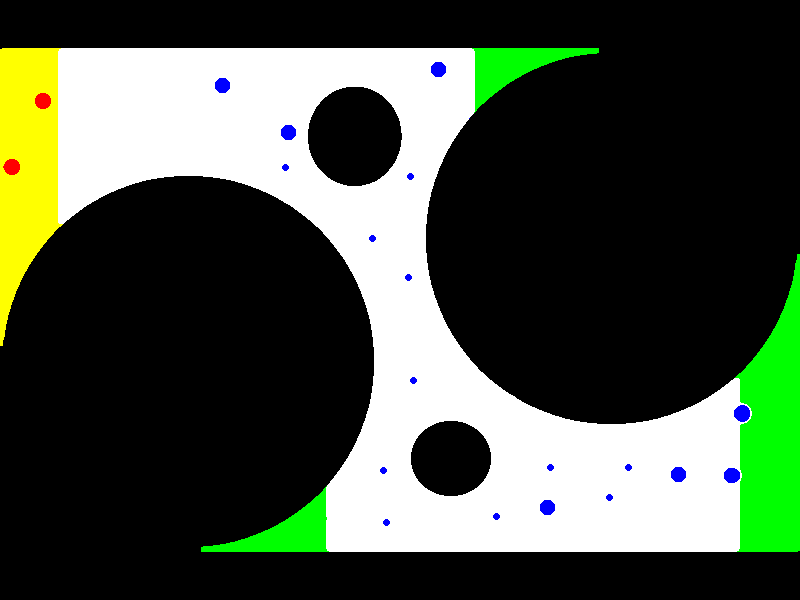
\includegraphics[width=65mm]{img/ImageProcessing/LevelImages/img_3.png} & 
\includegraphics[width=65mm]{img/ImageProcessing/LevelImages/img_5.png} \\
(a) & (b) \\[6pt]
  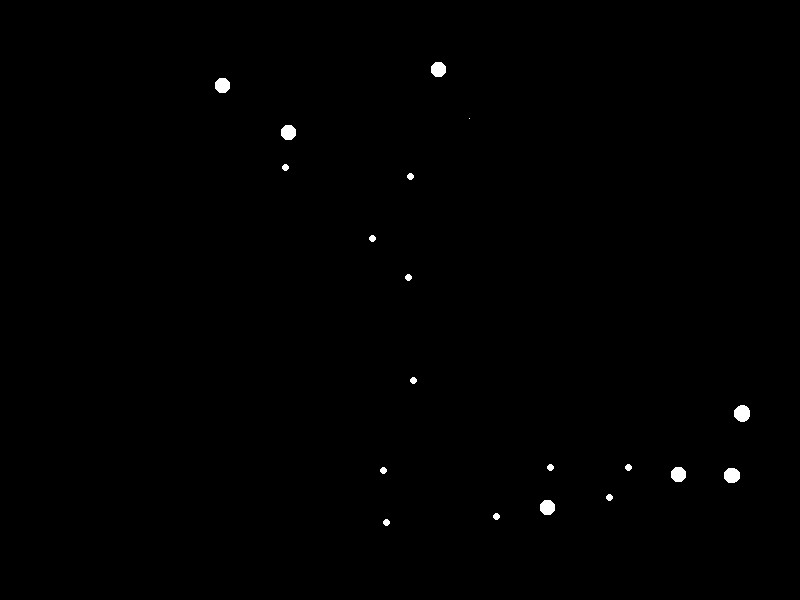
\includegraphics[width=65mm]{img/ImageProcessing/LevelImages/img_10.png} & 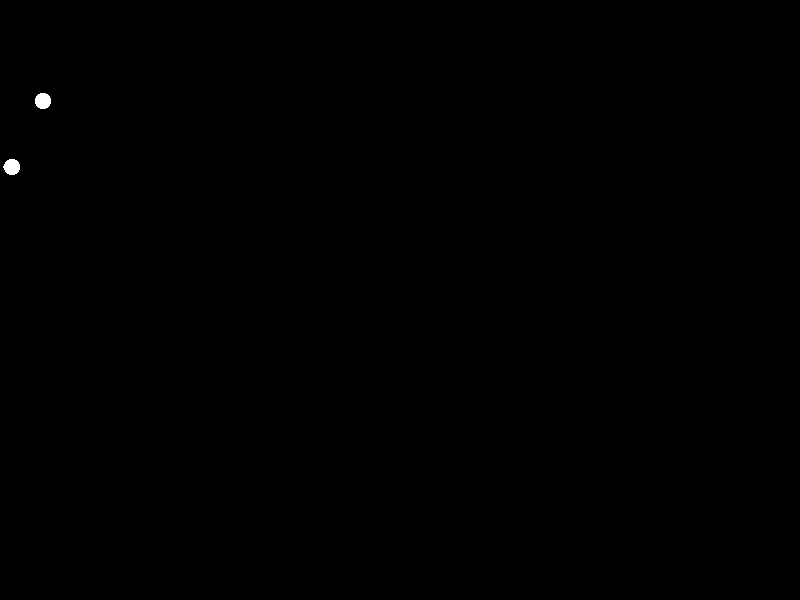
\includegraphics[width=65mm]{img/ImageProcessing/LevelImages/img_12.png} \\
(c) & (d) \\[6pt]
\end{tabular}
\caption{Various stages of processing the image. (a) After pre-processing, (b) image for \protect\lstinline|outerBorder| and \protect\lstinline|staticBodies|, (c) image for \protect\lstinline|rigidBodies|, and (d) image for \protect\lstinline|boatCenters|.\label{LevelImages}}
\end{figure}

The pre-processing brings the image in a state where information about the terrain can be easily extracted from it. Various information extraction techniques are applied to this processed image to obtain terrain information relevant to the simulation.

\begin{itemize}
	\item \textit{Sources}: Detected by a simple color comparison.
	\item \textit{Boats}: Boat pixels detected by color comparison. Their centers are located by a k-means analysis for 2 buckets. See Figure \ref{LevelImages}(d)
	\item \textit{Rigid Bodies}: The first step in the detection of the rigid body obstacles is the isolation of the obstacles as a binary "obstacle or not-obstacle" image. This is done by a series of boolean operations (provided in class \lstinline|utils|). This image is then supplied to the class \lstinline|PolygonHierarchy|.

The class \lstinline|PolygonHierarchy| is a recursive class holding two parameters: 
	\begin{itemize}
		\item \lstinline|data|: a set of points forming a closed polygon.
		\item \lstinline|subtree|: a vector of \lstinline|PolygonHierarchy|.
	\end{itemize}
The level of a \lstinline|PolygonHierarchy| indicates how many outer polygons enclose the polygons at that level. Note that the zeroeth-level \lstinline|data| is empty.

This \lstinline|PolygonHierarchy| is applied on Figure \ref{LevelImages}(c), and the first-level polygons give the rigid body obstacles.

	\item \textit{Fluid Domain}: The fluid domain is extracted in a similar manner by choosing the first-level polygon for Figure \ref{LevelImages}(b).

	\item \textit{Static Bodies}: The static bodies are detected by choosing the second-level polygons for Figure \ref{LevelImages}(b).

\end{itemize}
